%!TEX TS-program = pdflatexmk

% Copyright (c) 2018 - 2022, Martin Scheidt (ISC license)
% Permission to use, copy, modify, and/or distribute this file for any purpose with or without fee is hereby granted, provided that the above copyright notice and this permission notice appear in all copies.

\documentclass[border=2]{standalone}

\usepackage[dev]{tikz-trackschematic}

\begin{document}
  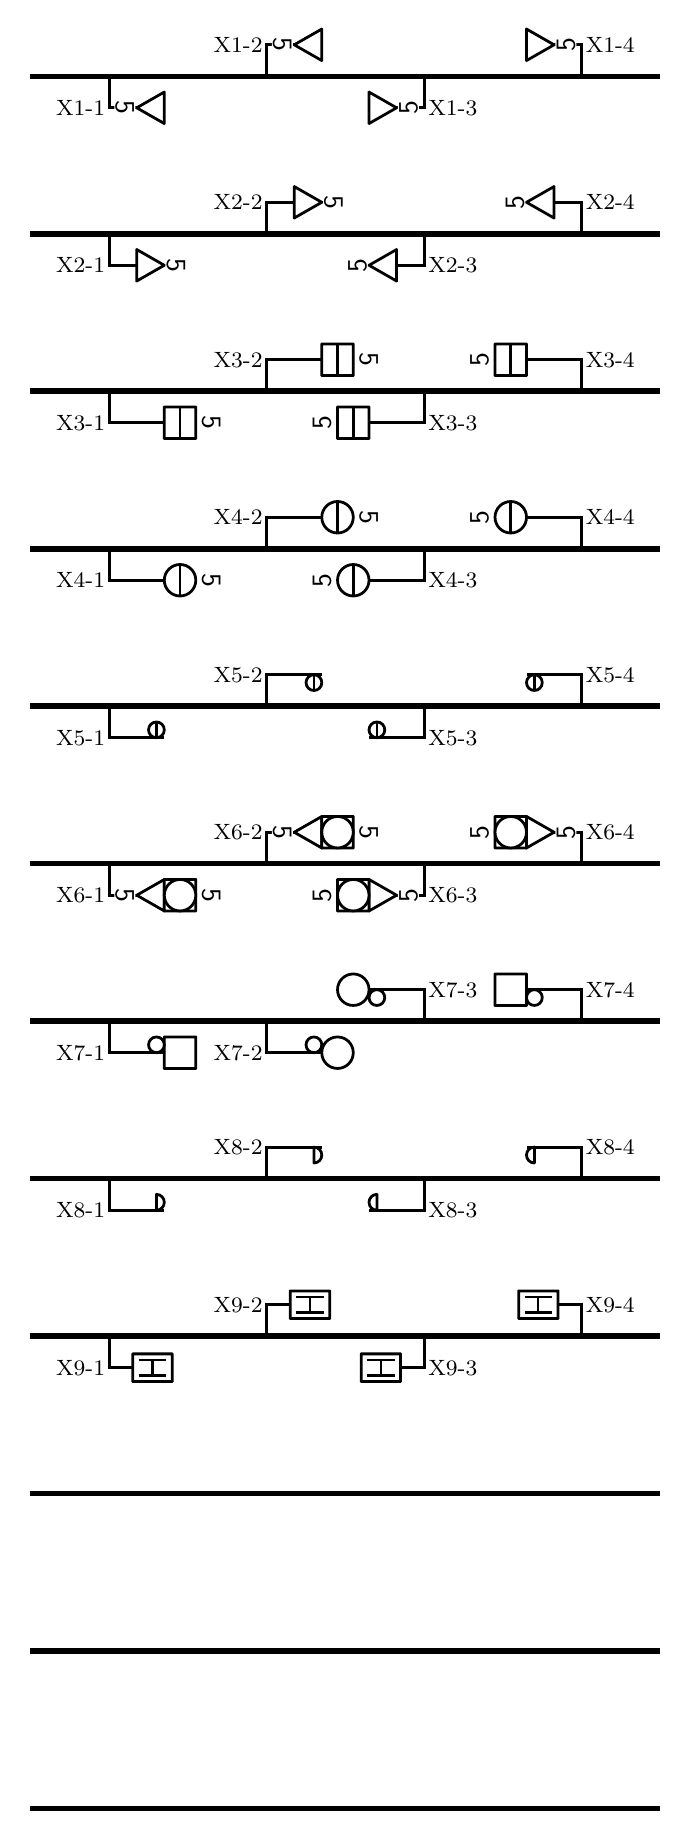
\begin{tikzpicture}

    \foreach \i in {1,2,...,12}{% base coordinate
      \coordinate (A\i) at ($(0,0) + 2*(0,-\i)$);% base coordinate
      \coordinate (B\i) at ($(8,0) + 2*(0,-\i)$);% base coordinate
    }

    \foreach \i in {1,2,...,12}{% draw main tracks on base coordinate
      \maintrack (A\i) --   (B\i);
    }

    \foreach \i in {1,2,...,12}{% coordinates for testing symbols
      \coordinate (X\i-1) at ($(1,0) + 2*(0,-\i)$);
      \coordinate (X\i-2) at ($(3,0) + 2*(0,-\i)$);
      \coordinate (X\i-3) at ($(5,0) + 2*(0,-\i)$);
      \coordinate (X\i-4) at ($(7,0) + 2*(0,-\i)$);
    }

    \distantsignal[forward ,distant speed=5] at (X1-1) label (X1-1);
    \distantsignal[forward ,distant speed=5,position=left] at (X1-2) label (X1-2);
    \distantsignal[backward,distant speed=5,position=left] at (X1-3) label (X1-3);
    \distantsignal[backward,distant speed=5] at (X1-4) label (X1-4);

    \speedsignal[forward ,speed=5] at (X2-1) label (X2-1);
    \speedsignal[forward ,speed=5,position=left] at (X2-2) label (X2-2);
    \speedsignal[backward,speed=5,position=left] at (X2-3) label (X2-3);
    \speedsignal[backward,speed=5] at (X2-4) label (X2-4);

    \blocksignal[forward ,locked,speed=5] at (X3-1) label (X3-1);
    \blocksignal[forward ,locked,speed=5,position=left] at (X3-2) label (X3-2);
    \blocksignal[backward,locked,speed=5,position=left] at (X3-3) label (X3-3);
    \blocksignal[backward,locked,speed=5] at (X3-4) label (X3-4);

    \routesignal[forward ,locked,speed=5] at (X4-1) label (X4-1);
    \routesignal[forward ,locked,speed=5,position=left] at (X4-2) label (X4-2);
    \routesignal[backward,locked,speed=5,position=left] at (X4-3) label (X4-3);
    \routesignal[backward,locked,speed=5] at (X4-4) label (X4-4);

    \shuntsignal[forward ,locked] at (X5-1) label (X5-1);
    \shuntsignal[forward ,locked,position=left] at (X5-2) label (X5-2);
    \shuntsignal[backward,locked,position=left] at (X5-3) label (X5-3);
    \shuntsignal[backward,locked] at (X5-4) label (X5-4);

    \signal[forward ,distant,block,route,distant speed=5,speed=5] at (X6-1) label (X6-1);
    \signal[forward ,distant,block,route,distant speed=5,speed=5,position=left] at (X6-2) label (X6-2);
    \signal[backward,distant,block,route,distant speed=5,speed=5,position=left] at (X6-3) label (X6-3);
    \signal[backward,distant,block,route,distant speed=5,speed=5] at (X6-4) label (X6-4);

    \signal[forward ,block,shunting] at (X7-1) label (X7-1);
    \signal[forward ,route,shunting] at (X7-2) label (X7-2);
    \signal[backward,route,shunting] at (X7-3) label (X7-3);
    \signal[backward,block,shunting] at (X7-4) label (X7-4);

    \shuntlimit[forward ] at (X8-1) label (X8-1);
    \shuntlimit[forward ,position=left] at (X8-2) label (X8-2);
    \shuntlimit[backward,position=left] at (X8-3) label (X8-3);
    \shuntlimit[backward] at (X8-4) label (X8-4);

    \berthsignal[forward ] at (X9-1) label (X9-1);
    \berthsignal[forward ,position=left] at (X9-2) label (X9-2);
    \berthsignal[backward,position=left] at (X9-3) label (X9-3);
    \berthsignal[backward] at (X9-4) label (X9-4);

  \end{tikzpicture}
\end{document}